%********************************************************************************************
%								COMANDOS ÚTILES PARA LATEX EN ESTE TP							
%
%	\ : espacio simple
%	\\ : nueva línea
%	\par : va a la línea de abajo y deja sangría
%	\vspace{##tamaño en pt##} o \vspace{\baselineskip} en general:
%								 para dejar un espacio vertical
%	\textbf{text} :text en negrita
%	\textit{text} :text en itálica
%
% GRAFICOS CENTRADOS:
%	\begin{center}
%		\includegraphics[width=\textwidth]{./img/##ruta imagen (no hace falta extension)##}
%	\end{center}
%		--> se pueden agregar atributos como scale por si se hace muy grande
%
% TABLAS CENTRADAS:
%	\begin{center}
%	\begin{tabular}{|c|c|}
%	\hline
%	\ \textbf{Programa} & \textbf{Ticks} \\
%	\hline
%		ASM & 675127609 \\
%	\hline
%	\end{tabular}
%	\end{center}
%
% ALGORITMOS (EN VARIOS LENGUAJES):
% \begin{lstlisting}
%	void sumoDiez(int &num)
%	{
%	    num += 10;
%	}
%	
%	int main()
%	{
% 	   int i;
%	    int numeroAProcesar = 20;
%	    for (i = 0; i < 50; i++)
%	    {
%	        sumoDiez(numeroAProcesar);	//Proceso el numero en cada ciclo
%	    } 
%	    return 0;
%	}
%	\end{lstlisting}
%
% para info sobre todo lo que tiene el package detallado:
% http://en.wikibooks.org/wiki/LaTeX/Source\_Code\_Listings
%
%********************************************************************************************

\documentclass[10pt,a4paper]{article}
\usepackage[utf8]{inputenc} % para poder usar tildes en archivos UTF-8
\usepackage[spanish]{babel} % para que comandos como \today den el resultado en castellano
\usepackage{a4wide} % márgenes un poco más anchos que lo usual
\usepackage[conEntregas]{caratula}
\usepackage{amssymb}
\usepackage{fancybox}
\usepackage[usenames,dvipsnames]{color}
\usepackage{hyperref}
\usepackage{listings}
\usepackage{ulem}
\usepackage{color}
\usepackage[table]{xcolor}
\usepackage{amsmath}
\usepackage{float}
\usepackage{pdflscape}
\usepackage[landscape]{geometry}

\hypersetup{
    colorlinks,
    citecolor=black,
    filecolor=black,
    linkcolor=black,
    urlcolor=black
}

\lstdefinestyle{customc}{
  belowcaptionskip=1\baselineskip,
  breaklines=true,
  frame=L,
  xleftmargin=\parindent,
  language=C,
  showstringspaces=false,
  basicstyle=\footnotesize\ttfamily,
  keywordstyle=\bfseries\color{green!40!black},
  commentstyle=\itshape\color{purple!40!black},
  identifierstyle=\color{blue},
  stringstyle=\color{orange},
}

\lstset{escapechar=@,style=customc}


\newcommand{\pk}[1]{\textbf{\textcolor{PineGreen}{\underline{{#1}}}}}

\newcommand{\fk}[1]{\textbf{\textcolor{red}{\dashuline{{#1}}}}}
\newcommand{\nullableFk}[1]{\textbf{\textcolor{YellowOrange}{\dashuline{{#1}}}}}

\newcommand{\nullableAtribute}[1]{\textbf{\textcolor{MidnightBlue}{{#1}}}}

\begin{document}

\titulo{Trabajo Práctico 1}
%\subtitulo{}

\fecha{\today}

\materia{Bases de Datos}
\grupo{Grupo 5}

\integrante{Barbeiton, Nicolás}{147/10}{nicolasbarbeiton@gmail.com}
\integrante{Chapresto, Matias Nahuel}{201/12}{matiaschapresto@gmail.com}
\integrante{Garassino, Agustín Javier}{394/12}{ajgarassino@gmail.com}
\integrante{Vileriño, Silvio}{106/12}{svilerino@gmail.com}

\maketitle

\tableofcontents
\newpage

\section{Introducción}

\section{Desarrollo}
\subsection{Diagrama Entidad-Relacion}
	\begin{figure}
	  \centering	
		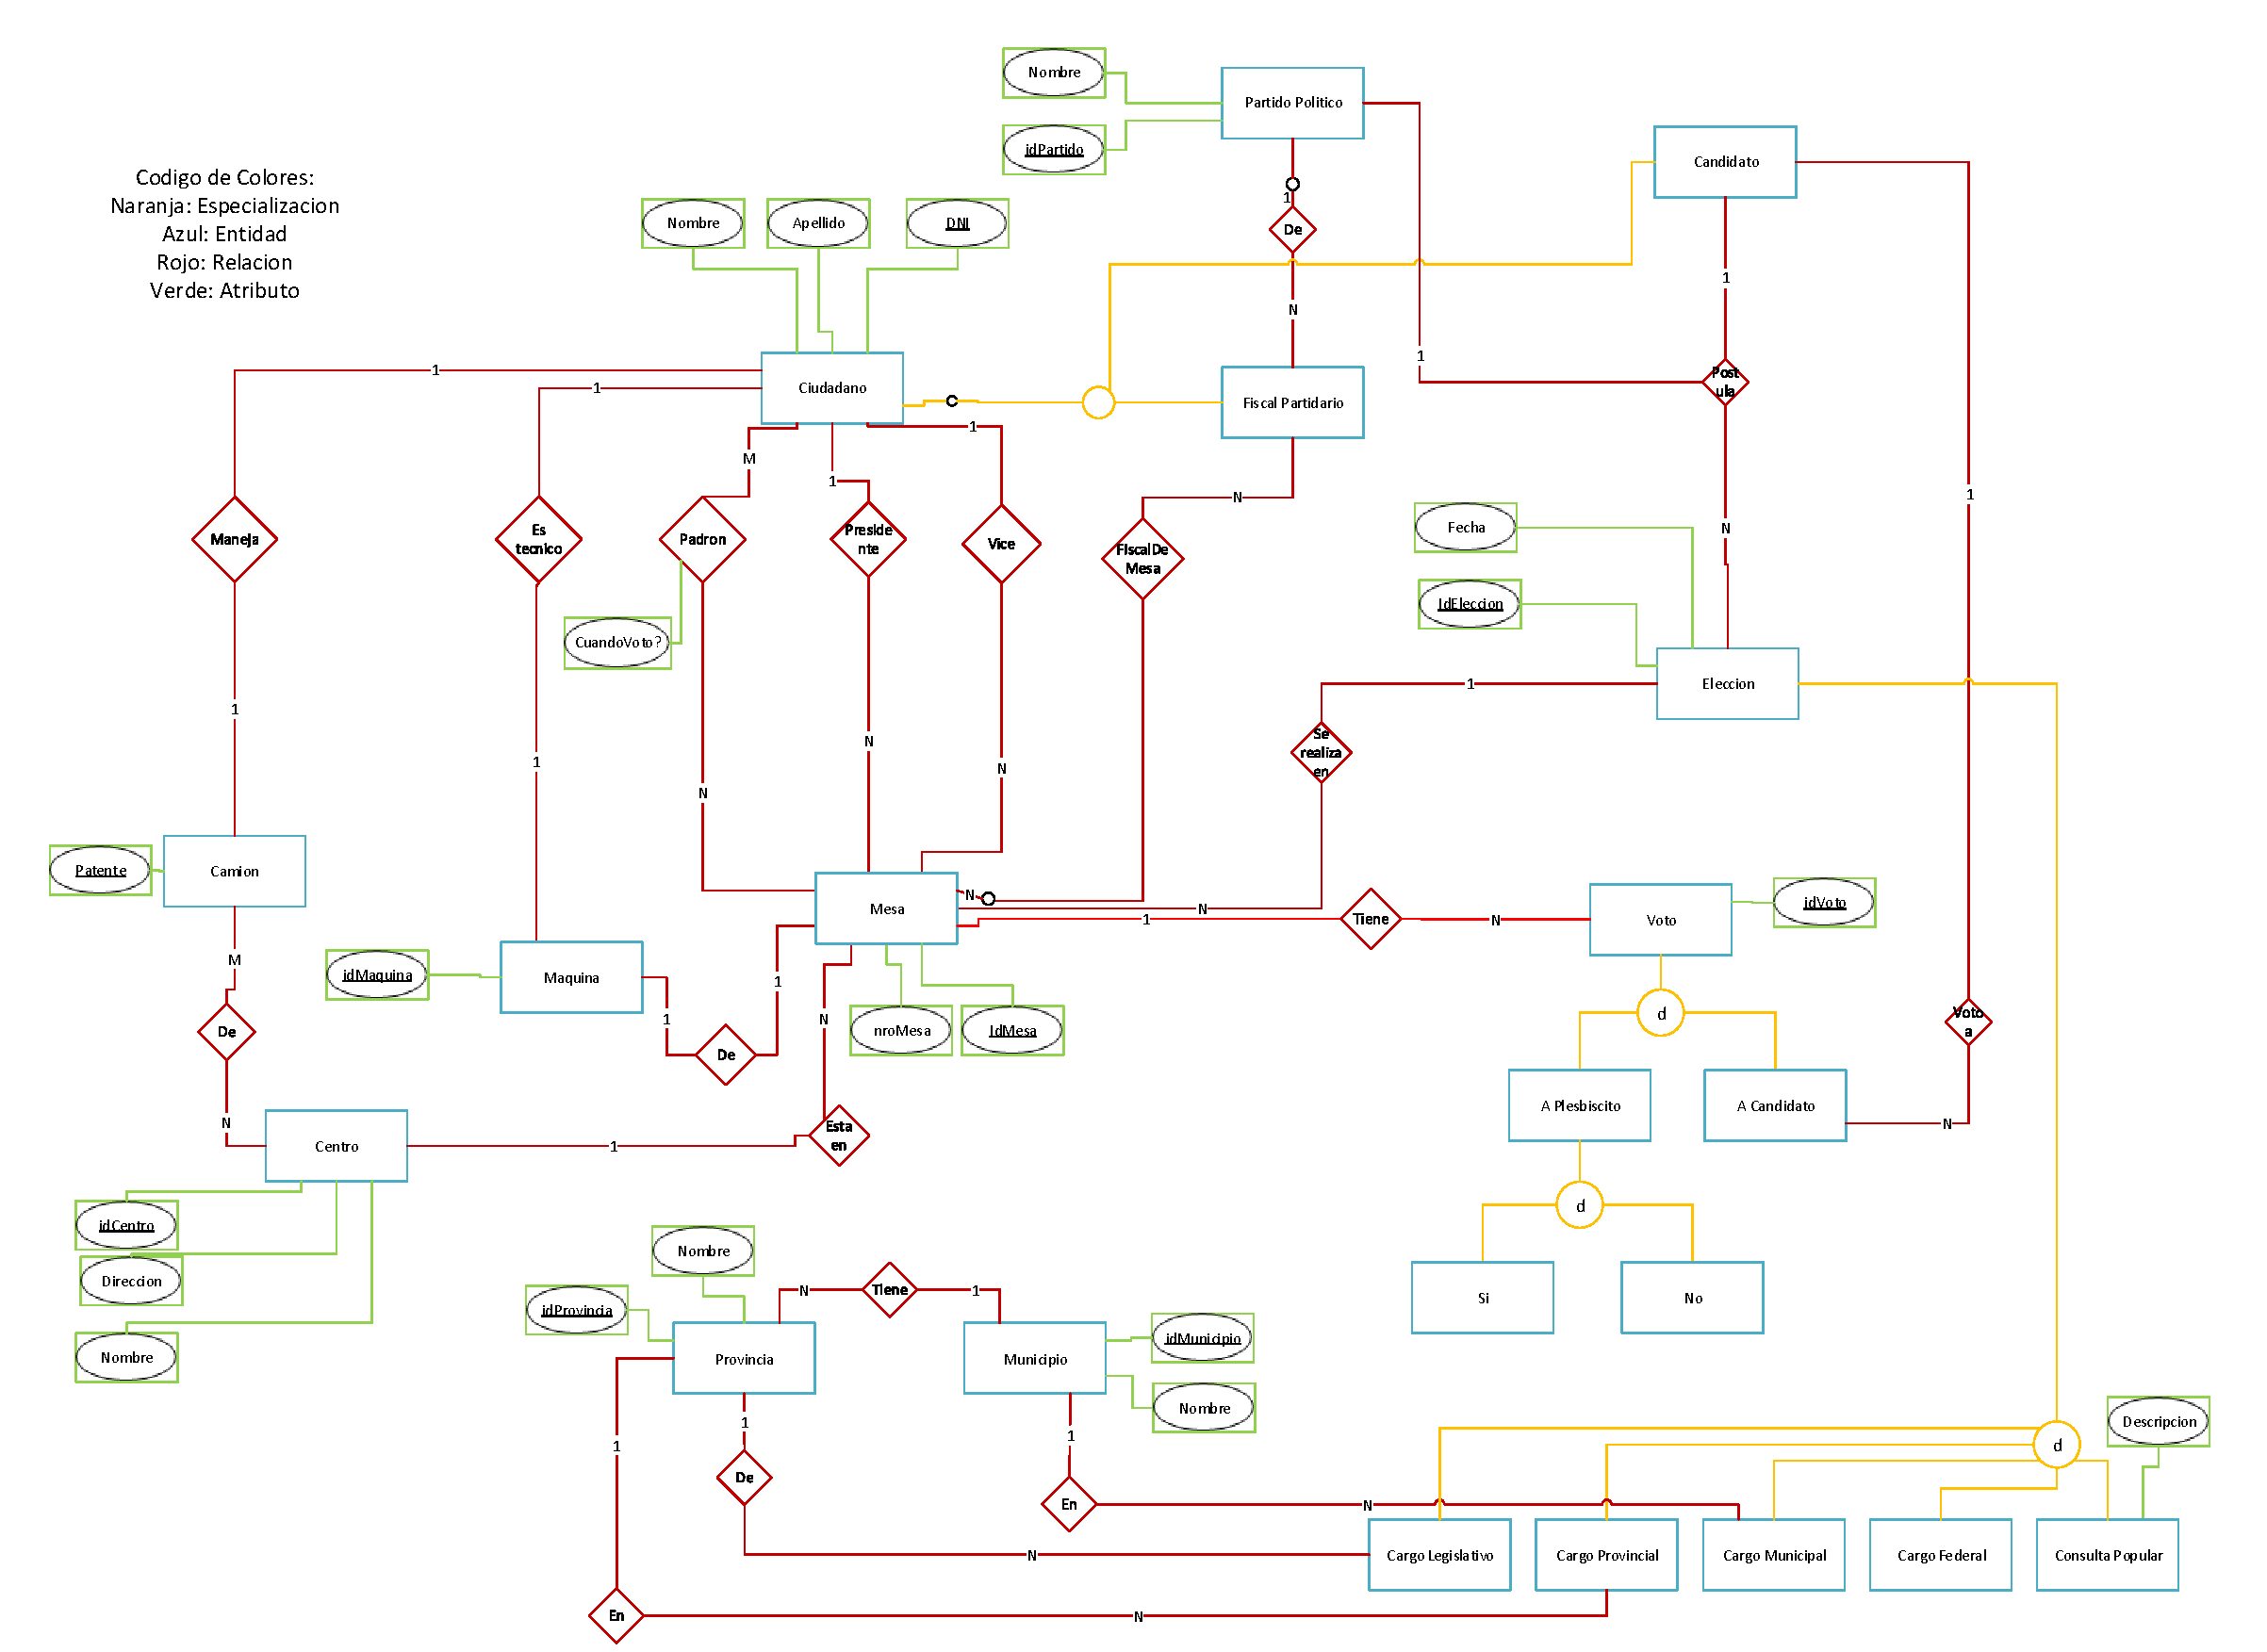
\includegraphics[scale=0.50]{fig/der.pdf}
	  \caption{Diagrama Entidad Relacion.}
	\end{figure}
\newpage

Restricciones Adicionales:

- Para cada persona que vota se debe insertar un voto(sin informacion de la persona) y actualizar correctamente la fecha y hora en la que voto y poniendo el “sello” virtual en el padron asignando un valor no nulo a cuandoVoto.

- La suma de los votos de todas las mesas de todos los candidatos debe ser menor o igual(votos en blanco diferencia) a la cantidad de ciudadanos que tiene el timestamp cuandoVoto? No nulo en el padron de dicha eleccion. (notar que esto tambien lo acota por la cantidad de ciudadanos)

- Todos los candidatos que se postulan para una eleccion, deben postularse para el mismo cargo.

- Asumimos que cada partido politico presenta un solo candidato.

- Los votos para una eleccion son: o bien consulta popular o bien de tipo candidato según corresponda el tipo de eleccion

-Si la eleccion es una consulta popular, los votos deben ser si/no. Sino, deben ser candidatos

-Un voto a candidato tiene que ser a un candidato que este postulado

- Un fiscal no puede estar en mas de una mesa en una eleccion

Habria que agregar como restriccion al der que un ciudadano no pueda ser tecnico, conductor, fiscal, etc en una misma eleccion.
\subsection{Modelo Relacional}

\textbf{Notacion:}
\begin{itemize}
	\item \pk{Primary Key} 
	\item \fk{Not Nullable Foreign Key}
	\item \nullableFk{Nullable Foreign Key}
	\item Not Nullable Atribute
	\item \nullableAtribute{Nullable Atribute}
\end{itemize}

\vspace{2mm}
\textbf{Entidades:}
\vspace{1mm}

\begin{itemize}
	\item \textbf{Eleccion} (\pk{idEleccion}, Fecha, Tipo) 
	\begin{itemize}
		\item PK = CK = \{idEleccion\}
	\end{itemize}
	\vspace{1mm}

	\item \textbf{Eleccion\_Consulta\_Popular} (\pk{\fk{idEleccion}}, Descripcion) 
	\begin{itemize}
		\item PK = CK = FK = \{idEleccion\}
	\end{itemize}
	\vspace{1mm}

	\item \textbf{Provincia} (\pk{idProvincia}, Nombre) 
	\begin{itemize}
		\item PK = CK = \{idProvincia\}
	\end{itemize}
	\vspace{1mm}

	\item \textbf{Municipio} (\pk{idMunicipio}, Nombre, \fk{idProvincia}) 
	\begin{itemize}
		\item PK = CK = \{idMunicipio\}
		\item FK = \{idProvincia\}
	\end{itemize}
	\vspace{1mm}


	\item \textbf{Eleccion\_Cargo\_Municipal} ((\fk{\pk{idEleccion}}, \fk{idMunicipio}) 
	\begin{itemize}
		\item PK = CK = \{idEleccion\}
		\item FK = \{idEleccion, idMunicipio\}
	\end{itemize}
	\vspace{1mm}

	\item \textbf{Eleccion\_Cargo\_Provincial} ((\fk{\pk{idEleccion}}, \fk{idProvincia}) 
	\begin{itemize}
		\item PK = CK = \{idEleccion\}
		\item FK = \{idEleccion, idProvincia\}
	\end{itemize}
	\vspace{1mm}

	\item \textbf{Eleccion\_Cargo\_Legislativo} ((\fk{\pk{idEleccion}}, \fk{idProvincia}) 
	\begin{itemize}
		\item PK = CK = \{idEleccion\}
		\item FK = \{idEleccion, idProvincia\}
	\end{itemize}
	\vspace{1mm}
	 

	\item \textbf{Voto} (\pk{idVoto}, \fk{idMesa}, Tipo) 
	\begin{itemize}
		\item PK = CK = \{idVoto\}
		\item FK = \{idMesa\}
	\end{itemize}
	\vspace{1mm}

	\item \textbf{Voto\_A\_Candidato} (\pk{idVoto}, \fk{DNI}) 
	\begin{itemize}
		\item PK = CK = \{idVoto\}
		\item FK = \{idVoto, DNI (references Candidato on DNI)\}
	\end{itemize}
	\vspace{1mm}

	\item \textbf{Ciudadano} (\pk{DNI}, Nombre, Apellido, \fk{idMesa}, \nullableAtribute{selloVoto}) 
	\begin{itemize}
		\item PK = CK = \{DNI\}
		\item FK = \{idMesa\}
		\item \textbf{Nota:} selloVoto es de tipo fecha/hora, puede ser nulo y por defecto comienza siendo nulo.
	\end{itemize}
	\vspace{1mm}


	\item \textbf{Fiscal\_Partidario} (\pk{DNI}, \fk{idPartido}) 
	\begin{itemize}
		\item PK = CK = \{DNI\}
		\item FK = \{idPartido\}
	\end{itemize}
	\vspace{1mm}

	\item \textbf{Candidato} (\pk{\fk{DNI}}) 
	\begin{itemize}
		\item PK = CK = \{DNI\}
		\item FK = \{DNI references Ciudadano on DNI\}
	\end{itemize}
	\vspace{1mm}


	\item \textbf{Partido\_Politico} (\pk{idPartido}, Nombre) 
	\begin{itemize}
		\item PK = CK = \{idPartido\}
	\end{itemize}
	\vspace{1mm}

	\item \textbf{Camion} (\pk{Patente}, \fk{idConductor}) 
	\begin{itemize}
		\item PK = CK = \{Patente\}
		\item FK = \{idConductor (references Ciudadano on DNI)\}
	\end{itemize}
	\vspace{1mm}

	\item \textbf{Centro} (\pk{idCentro}, Nombre\_Establecimiento, Direccion) 
	\begin{itemize}
		\item PK = CK = \{idCentro\}
	\end{itemize}
	\vspace{1mm}

	\item \textbf{Maquina} (\pk{idMaquina}, \fk{idMesa}, \fk{idTecnico}) 
	\begin{itemize}
		\item PK = CK = \{idMaquina\}
		\item FK = \{idMesa, idTecnico (references Ciudadano on DNI)\}
	\end{itemize}
	\vspace{1mm}

	\item \textbf{Mesa} (\pk{idMesa}, nroMesa, \fk{idPresidente}, \fk{idVicepresidente}, \fk{idEleccion}, \fk{idCentro}) 
	\begin{itemize}
		\item PK = CK = \{idMesa\}
		\item FK = \{idPresidente (references Ciudadano on DNI), idVicepresidente (references Ciudadano on DNI), idEleccion, idCentro\}
	\end{itemize}
	\vspace{1mm}

\end{itemize}
		
\vspace{2mm}
\textbf{Relaciones:}
\vspace{1mm}

\begin{itemize}
	
	\item \textbf{Camion\_Centro} (\pk{\fk{patente}, \fk{idCentro}}) 
	\begin{itemize}
		\item PK = CK = \{(patente, idCentro)\}
		\item FK = \{patente, idCentro\}
	\end{itemize}
	\vspace{1mm}

	\item \textbf{Fiscales} (\pk{\fk{DNI}, \fk{idMesa}}) 
	\begin{itemize}
		\item PK = CK = \{(DNI, idMesa)\}
		\item FK = \{idMesa, DNI  (references Ciudadano on DNI)\}
		\item \textbf{Nota:} Puede haber mesas sin fiscal. Mesa participa parcialmente en esta relacion.
	\end{itemize}
	\vspace{1mm}

	\item \textbf{Postulaciones} (\pk{\fk{idEleccion}, \fk{DNI}}, \fk{idPartido}) 
	\begin{itemize}
		\item CK = \{(idEleccion, DNI), (idEleccion, idPartido)\}
		\item PK = CK = \{(idEleccion, DNI)\}
		\item FK = \{idEleccion, idPartido, DNI (references Candidato on DNI)\}
	\end{itemize}
	\vspace{1mm}

\end{itemize}

\textbf{Notas:} 
\begin{itemize}
	\item Todos los atributos en negro son no nullables.
	\item Las \pk{Primary Keys} del modelo fisico, no son autoincrement(identity) por motivos de testing.
	\item Todas las relaciones son de participacion total salvo que se explicite lo contrario.
	\item En la doble especializacion de voto por la rama de consulta popular, consideramos innecesario crear la tabla A\_Plesbicito con el campo tipo que indica si el voto es por Si o por No, pues es mas sencillo directamente especializar en el nivel superior, que un voto puede ser de 3 tipos:
	\begin{itemize}
		\item A Candidato
		\item A Consulta Popular, A favor
		\item A Consulta Popular, En contra
	\end{itemize}


\end{itemize}




\section{Conclusiones}

\end{document}
